% !Mode:: "TeX:UTF-8"
\chapter*{中文译文}
\setcounter{equation}{0}
\par{反向传播算法((Rumelhart, Hinton, \& Williams, 1986)中对具有前反馈功能的神经网络中间层进行训练对于得到与输出想要结果相对应的输入向量来说是十分有用的。这种算法采用传播真实的输出和想要的输出之间的差异来计算某一个方向的权值的变化以便于去减少这种差异。在这篇文章里面,我们将介绍一种如何用反向传播的技术来学习那些没有被监督信号标记的输入向量的特征和约束。}
\par{如果所需的输出结果不明确,那么很显然机器不能够很明确的知道学习的目标是什么。我们在这里假定,学习的目标是在所观察到的数据中学习一些不同特征和约束也即是隐藏因子。这些隐藏因子可以用于随后的决策或者用高能量来表述的极不可能出现的数据载体。在这种网络中,对于输入向量$x$ 的可能性可以采用向量 的全局能量$E(x)$ 与所有可能输入向量$v$ 的能量的比值来表示。
\begin{equation}\label{equation1}p(x) = \frac{{{e^{ - E(x)}}}}{{\sum\nolimits_v {{e^{ - E(v)}}} }}\end{equation}
}

\par{直观地说,一个良好的无监督学习过程应该发现概率很高而且经常出现的隐性因素。这可以通过降低所观察到的数据向量的能量、提高的“负”的数据载体实现。这也就是能够发现可以用来构造好的数据模型的隐藏因子的模式。通过使用当前模型来生成一组负的数据向量,我们可以把无监督的学习任务转换为一种给观察数据赋予低能量而负数据的赋予高能量的监督学习过程。然而,要注意的是负数据向量要取决于当前的模型,它会随着模型的学习过程而有所改变。}
\par{
神经网络发现的特征和约束的质量可以用观察的数据的概率的对数和表示。对于单个向量的其对于整个和的贡献是:
\begin{equation}\label{equation2}\log p(x) =  - E(x) - \log \sum\limits_v {{e^{ - E(v)}}} \;\;\;\end{equation}
}

\par{这些特征和约束可以通过不断地调整不同神经元之间联系的权重来进行提升,以便于最大化观察数据的概率的对数。我们可以通过计算概率对数来表示相似度对数的梯度。
 \begin{equation}\label{equation3}\Delta {w_{ij}}{\kern 1pt} {\kern 1pt} {\kern 1pt}  \propto {\kern 1pt} {\kern 1pt} \frac{{\partial \log {\kern 1pt} p(x){\kern 1pt} {\kern 1pt} {\kern 1pt} }}{{\partial {w_{ij}}}} = {\kern 1pt}  - \frac{{\partial E(x){\kern 1pt} {\kern 1pt} {\kern 1pt} }}{{\partial {w_{ij}}}}{\kern 1pt}  + {\kern 1pt} {\kern 1pt} \sum\nolimits_v {p(v)\frac{{\partial E(v){\kern 1pt} {\kern 1pt} {\kern 1pt} }}{{\partial {w_{ij}}}}} \;\end{equation}
其中 ${{\rm{w}}_{{\rm{ij}}}}$ 是第 $i$ 层神经元到$j$  层神经元之间联系的权重。}
	\par{第一项很容易计算。我们假设对于每一个神经元 $j$对来自其下一层的神经元$i$ 进行加权求和得到总输出为${z_j} = {\kern 1pt} {\kern 1pt} \sum\nolimits_i {{y_i}{w_{ij}}} $ ,其中如果${y_i}$ 是输入层的话,那么${x_i}$ 和${y_i}$ 相等。平滑非线性函数 ${z_j}$用于计算这个神经元${y_j}$ 的活动量。每一个神经元的能量可以用任意平滑函数来表示。在这篇文章里,我们用两层非线性隐藏神经元,而且能量由第二个隐藏层决定的计算由公式(\ref{equation4})表示。
 \begin{equation}\label{equation4}E(x)\; = \;\sum\limits_j {{\lambda _j}\log (1 + y_j^2)} \;\end{equation}
在这里 ${y_j}$是神经元$j$在第二个隐藏层的活动量, ${\lambda _j}$是通过对比反向传播方法学习到的尺度参数。这种“重尾”的能力计算对于构造恰当的约束来说是有益处的。在自然风景的图像中,比如说一个本地面向边缘的滤波器会得到一个几乎所有的点都是0 的输出。很少会出现输出偏离0的情况,但是,这个也许会功能很强大,所以这种侵犯分布是非常non-Gaussian的。通过用等式4中的能量计算,我们希望这个网络能够找到一种类型的约束来对数据分布进行建模。}
\par{通过网络进行直传来计算所有单位的活动量之后,我们做一个由Rumelhart在1986 年提出的后向传播的实验。后向传播使用链式法则来计算对于每一个连接的权重 $\frac{{\partial E(x){\kern 1pt} {\kern 1pt} {\kern 1pt} }}{{\partial {w_{ij}}}}$ ,通过一路反向传播直到结束,对于输入向量每一个分量 ${x_i}$我们可以计算出$\frac{{\partial E(x){\kern 1pt} {\kern 1pt} {\kern 1pt} }}{{\partial {x_i}}}$ 。}
\par{不幸的是,公式\ref{equation3}中的第二个式子比较难于处理。它涉及到从所有可能的数据向量的导数的加权平均值,因此除了一些特殊情况以外,它不能有效地计算出来。然而我们通常希望这个平均值由每一个可以感知得到的小的分量确定,所以通过在相当小数量的数据样本上来计算 $\frac{{\partial E(x){\kern 1pt} {\kern 1pt} {\kern 1pt} }}{{\partial {w_{ij}}}}$的平均值来估计其分布$p\left( . \right)$  似乎是合理的。一种方法是运行一个具有热噪声的物理过程的马尔可夫链来得到这些样本。如果我们把数据空间看作是是水平面的话,那么我们可以把每一个数据的势能作为高,神经网络通过高和很容易计算的梯度来决定一个潜在的势能面。我们可以想象粒子在该表明沿着下坡方向移动,但是也会由于附加的高斯噪声而抖动。经过一定的步数之后,分子会丢失来自开始地方的所有信息。如果我们使用足够小的步间隔,它在数据空间中所有可能出现的地方服从Boltzmann分布。这种构造样本的过程缓慢而又痛苦,而且即使最后得到需要的分布,由抽样产生的差异也有可能会掩盖真正的学习信号。}
\par{相当令人惊讶地是,模拟的物理过程达到平衡分布的条件是不必要的。如果我们在观测数据向量上开始这个过程,只要运行几步,我们就可以生成可以很好地调节权重的一个“虚构样本”(Hinton, 2002).) 。直观地说,如果该马尔科夫链以一个系统的方式将数据发散,现在已经有证据表明,该模型是不完美的,并且它可以通过降低初始数据矢量的能量和提高虚构的能量来改善(在数据空间的这个局部区域)。这在理论上是可行的,因为这个学习过程会导致模型给那些远离任何数据的向量所在的未访问的数据空间区域以低能量。然而,这种学习方法在大量的数据上运行良好的事实表明,这个理论不足于拒绝学习这个学习过程,就如同局部极小的存在使得不能够拒绝反向传播。}
\par{对比反向传播学习过程周期通过对以下公式对观察到的数据的权重进行调整:  \begin{equation}\label{equation5}\Delta {w_{ij}} = \eta \;\left( { - \frac{{\partial E(x){\kern 1pt} {\kern 1pt} {\kern 1pt} }}{{\partial {w_{ij}}}}{\kern 1pt}  + {\kern 1pt} {\kern 1pt} \frac{{\partial E(\mathop x\limits^ \wedge  ){\kern 1pt} {\kern 1pt} {\kern 1pt} }}{{\partial {w_{ij}}}}} \right){\kern 1pt} \;\;\end{equation}
其中$\eta$ 是学习速率而 $\mathop x\limits^ \wedge $ 是由其实向量$x$ 得到的虚构向量。势能面的梯度通过噪声的形式来影响 。}
	\par{为了更好地阐述这个学习过程,我们在把它应用在一个模拟的具有五个刚性连接和五个球状的关节的三维手臂以用于探索非线性的运动约束。第一个球状关节连接到手臂的原始部分,每一个数据向量包括15个用于保留链接点的笛卡尔坐标。很显然这些15维的坐标只有10维的自由度因为其中的5维由5个关节点连接构成。这些约束的格式如\ref{equation6}:
 \begin{equation}\label{equation6}
{\left( {{x_i} - {x_{i + 1}}} \right)^2} + {\left( {{y_i} - {y_{i + 1}}} \right)^2} + {\left( {{z_i} - {z_{i + 1}}} \right)^2} - {l_{i,i + 1}}^2 = 0\;\;
 \end{equation}

其中 $i$$i + 1$ 和 是邻接节点的索引,而 ${l_{i,i + 1}}$是两个连接之间的长度,由于这些约束是高度非线性的,所以线性维度的降维过程类似于主成分分析,而不是因子分析。}
\par{我们采用了一个具有15个神经元和两个隐藏层的神经网络。第一个隐藏层计算输入向量的加权平均值的平方。顶层中五个单元每一个计算前述的平方的权重和并且与学习偏差相加。很显然如果具有正确的权重和偏差,每一个层都可以实现公式6中当且仅当约束完全满足,输出结果为0的约束.问题是仅仅通过观察数据能否得到恰当的权值和偏差。}
\par{在这个例子中,第一个隐藏层不贡献能量,第二个隐藏层以 ${\lambda _j}\log (1 + y_j^2)$贡献能量。这重尾的函数采用非零输出结果惩罚顶层单元,但是如若输出已经很大,改变输出对这种惩罚鲜有影响。}
\par{图1显示了由对比反向传播算法学习得到的权重和顶层偏差。对于每一个邻近的连接点,第一个隐藏层中有三个神经元来学习计算两节点坐标间的差异。这些差异经常在三个正交方向上计算。在第二隐层中的每个单元学习了五个约束的线性组合,但它使用的权重与每个约束的三次微分同阶,由此它可以通过使用其偏差确切的消去三次微分的定和。}
\par{当每个数据向量中随机百分之十的输入变量缺失同样的网络也可以学习五个约束。缺失的输入变量可作为额外参数,初始化为随机值,由公式\ref{equation5}所示的模式学习,${w_{ij}}$ 替换为${x_i}$ 。这些随机输入意味着每个实例的约束在学习起初只有的 ${.9^6} = 0.53$ 概率满足。但是,重尾能量函数意味着强烈违反约束仅仅会贡献很小的梯度,即是说学习过程会被精确满足约束所驱使。}
\par{我们同样在对学习更具挑战性的任务上应用相似的神经网络,其允许我们简洁的描述小片自然风光数字图像的序列统计结构。在此任务上,我们用如前所述的同样的网络层结构,激活函数和能量函数,不同的是此网络在输入层具有256个单元,在两个隐层的每层都有400单元。我们同样在每个隐层中排列这些单元在$20 \times 20 $的方格上,并在图形上限制了其连通性,以使得第一隐层每个单元仅可以连接第二隐层同样网格位置的单元和其24近邻。
\begin{figure}[htbp]
\centering
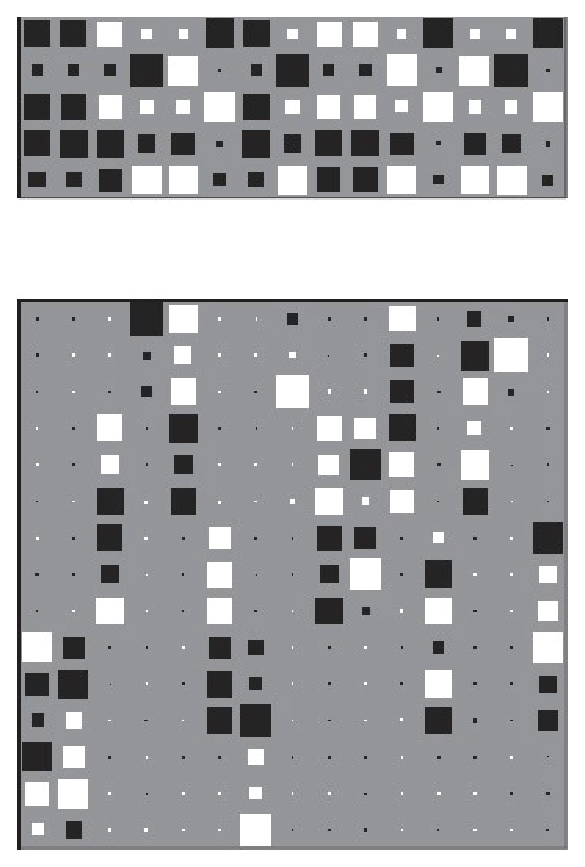
\includegraphics[width=0.4\textwidth]{deeplearning.eps}
\label{fig:deeplearning}
\vspace{\baselineskip} % 表示图与正文空一行
\end{figure}}
\par{
\footnotesize
 Fig.\ref{fig:deeplearning},矩形的白点和黑点代表通过网络学习到的正负权重的值。每一列的下部分表示从${x_1},{\rm{ }}{y_1},{\rm{ }}{z_1},{\rm{ }}{x_2},{\rm{ }}{y_2},{\rm{ }}{z_2} \ldots {x_5},{\rm{ }}{y_5},{\rm{ }}{z_5}$ 连接点学习到的连接权值。比如说,在第一、第二、第七列中展示了可以用于计算两个连接点之间的三维正交距离平方的神经元的权重。在每一行的上部分表示从第一个隐藏层到第二个隐藏层之间的权重。比如说第一个隐藏层的第一个、第二个、第七个单元中和第三行的神经元具有相同的负权重。这些权重以一些非常小的随机值开始,并3300次通过800个随机胳膊构成的连接长度为1 的训练集。每训练100 次,权重更新一次。为了消除不必要的权重,每一加上了朝着权重变化方向加了0.0002的衰减. 在乘上学习比例 ${\eta _{ij}}$(以0.0001为起始值)之前, $\Delta {w_{ij}}$由公式(\ref{equation5}) 来确定。如果 $\Delta {w_{ij}}$和它先前的值的信号相符合那么 ${\eta _{ij}}$以1\% 的速度增加,否则以5\% 的速度减少。为了进一步加快学习,而不会造成发散振荡,各权重的更新是其上一次更新速度的0.9 倍。}

\par{图二展示了用这个模型学习到的一些特征。第一层的神经元自己学习一个具有连通性、定向性的新的图像片段特征。这些特征有着和在大多数哺乳动物的初级视觉层次中发现的简单感知细胞有着惊人相似度和自然图像中的统计结构特征也十分相似(Bell \&Sejnowski, 1997; Olshausen \& Field, 1996)。 第二层的神经元展现显示类似的反应偏好和空间频率。但是似乎对于输入层的空间相位不敏感。由于两个隐藏层之间的严格限制,方向局部连续性的地形图和空间频率构成了一个新的特征。}

